
\begin{enumerate}
    \item In the circuit shown, initially there is no charge on capacitors and keys \( S_1 \) and \( S_2 \) are open. The values of the capacitors are \( C_1 = 10 \mu F \), \( C_2 = 30 \mu F \) and \( C_3 = C_4 = 80 \mu F \). Which of the statement(s) is/are correct?
        \begin{tasks}(2)
        	\task At time \( t = 0 \), the key \( S_1 \) is closed, the instantaneous current in the closed circuit will be \( 25 mA \).
        	\task If key \( S_1 \) is kept closed for a long time such that capacitors are fully charged, the voltage across the capacitor \( C_1 \) will be \( 4 V \).
        	\task The key \( S_1 \) is kept closed for a long time such that capacitors are fully charged. Now key \( S_2 \) is closed, at this time, the instantaneous current across \( 30 \Omega \) resistor (between points \( P \) and \( Q \)) will be \( 0.2 A \) (round off to \( 1^{st} \) decimal place).
        	\task If key \( S_1 \) is kept closed for a long time such that capacitors are fully charged, the voltage difference between points \( P \) and \( Q \) will be \( 10 V \).
        \end{tasks}
\end{enumerate}
\begin{center}
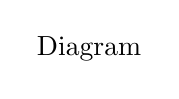
\begin{tikzpicture}
\node {Diagram};
\end{tikzpicture}
\end{center}
